In this section, we discuss the determination of the MVA shape of $\Wjets$ 
background in the MVA analysis and its associated systematic uncertainties. 

When we set the upper limits using the MVA shape, referred to as the shape 
analysis, the MVA distribution for $\Wjets$ background is estimated 
in a data-driven method as described below. 
\begin{enumerate}
\item  We select the $\Wjets$ enriched side band in data, which contains events 
with one lepton pass the full selection and the other fail the full selection 
but pass the lepton FO selection. We use the version ``V4'' of electron FO 
and version ``M2'' for muon FO, defined in Section~\ref{sec:bkg_fakes}.
\item We estimate the contributions from other SM backgrounds 
(such as $WW$, $\ttbar$, $tW$ etc.) in this side band region using MC.
\item We then weight the $\Wjets$ events in the side band region in data, subtracting the 
other SM background contributions, by the $FR/(1-FR)$ where FR is the fakerate measured in data.
\item The nominal $\Wjets$ MVA shape is then determined from these FR weighted events.
\end{enumerate}

To validate this data-driven method we perform a closure test in MC in the 0-jet bin. 
In this test, we use the fakerate derived from QCD MC to estimate the $\Wjets$ MVA shape in $\Wjets$ MC. 
We then compare the predicted MVA distribution using this data-driven method with the one 
obtained directly from the signal region in MC. Figure~\ref{fig:wjetsshape_mcclosure} 
shows the comparison done with various higgs selections. 
Overall we find the difference in the $\Wjets$ MVA distribution 
between the data-driven method using the side band region and the 
prediction in the signal region within 20\% for all the higgs selections. 
Given that we have an overall uncertainty on the 
$\Wjets$ yield about $35\%$, the uncertainties due to the shape is expected to the sub-dominant. 
These uncertainties are included taken in the upper limits reported in Section~\ref{sec:dataresults}.
%%%%%%%%%%%%%%%%%%%%%%%%%%%%%%%%%%%5
\begin{figure}[!htbp]
\begin{center}
\subfigure[mH = 115]{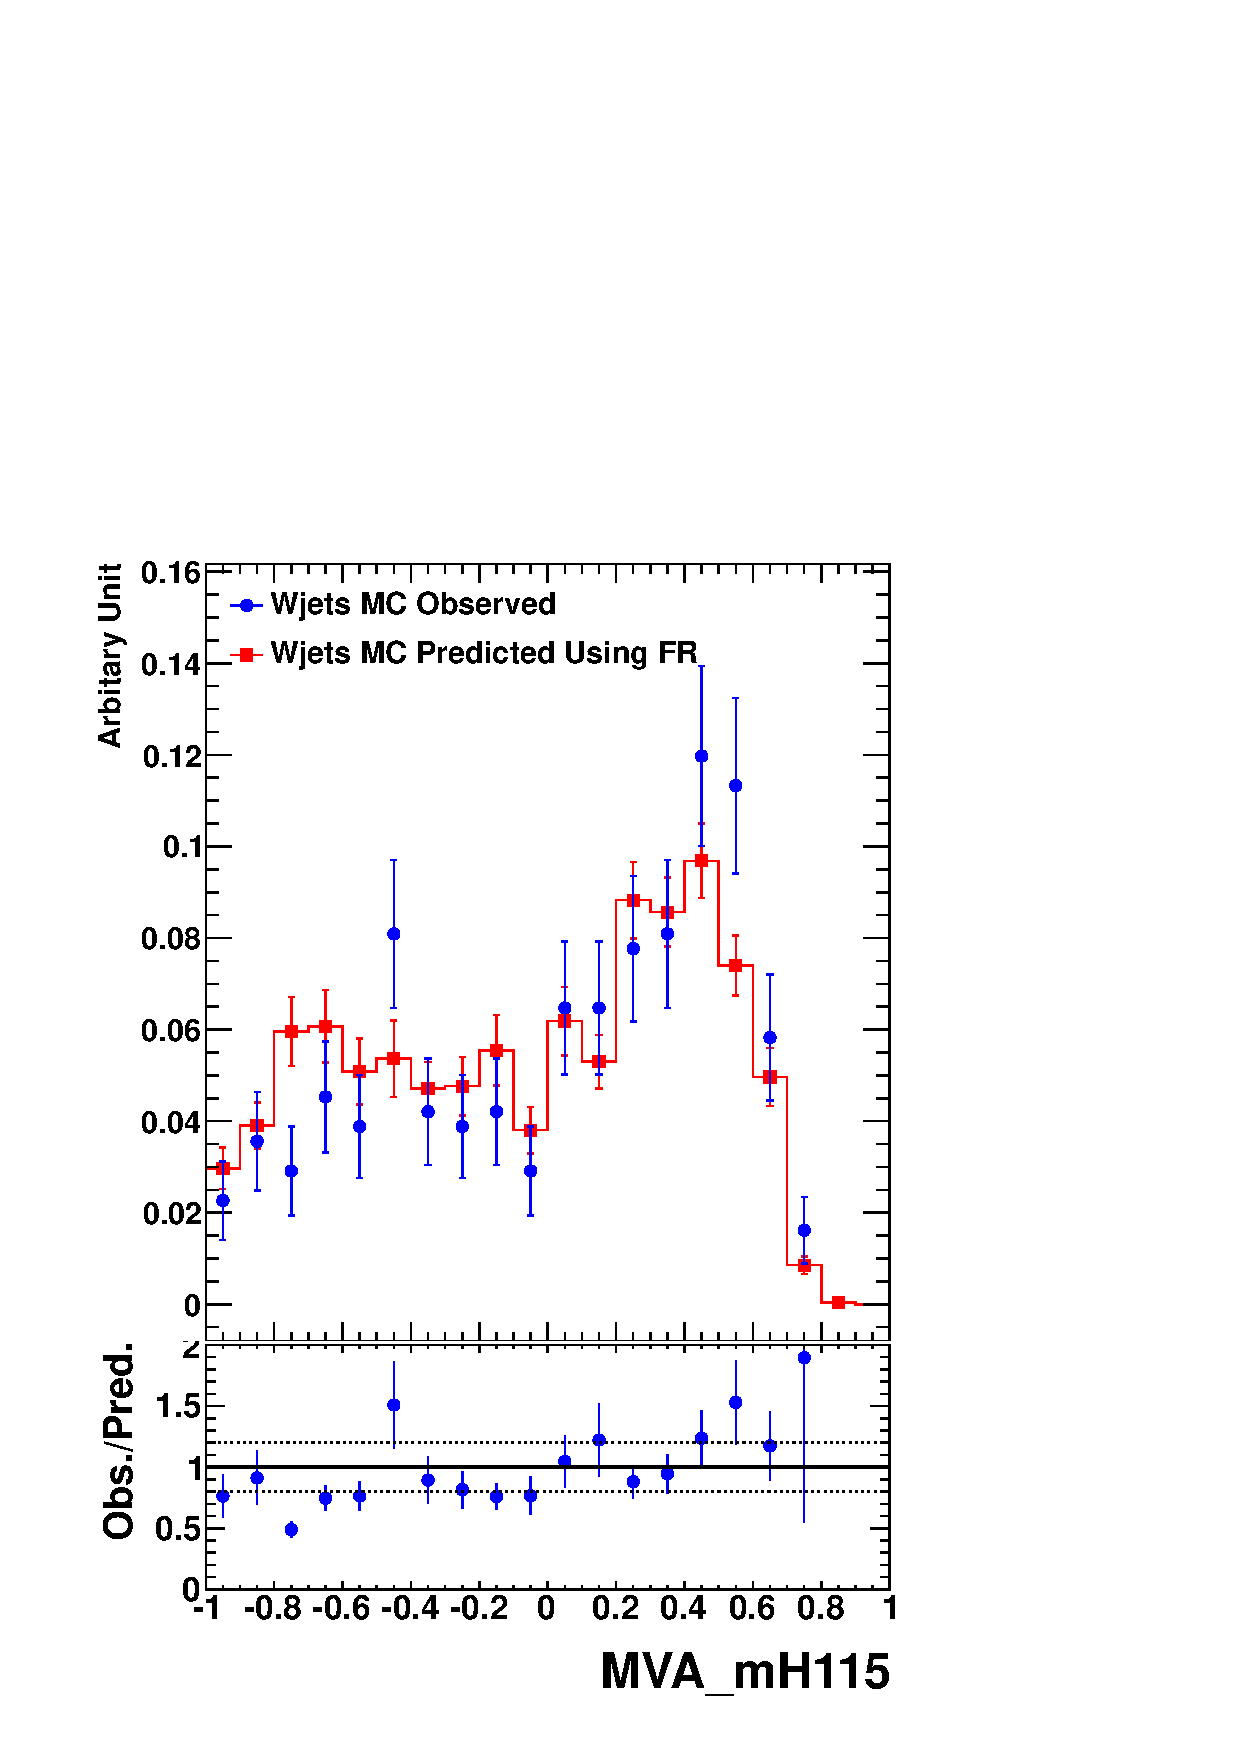
\includegraphics[width=0.3\textwidth]{figures/Wjets_MVA_MCClosure_mH115_0Jet.pdf}}
\subfigure[mH = 130]{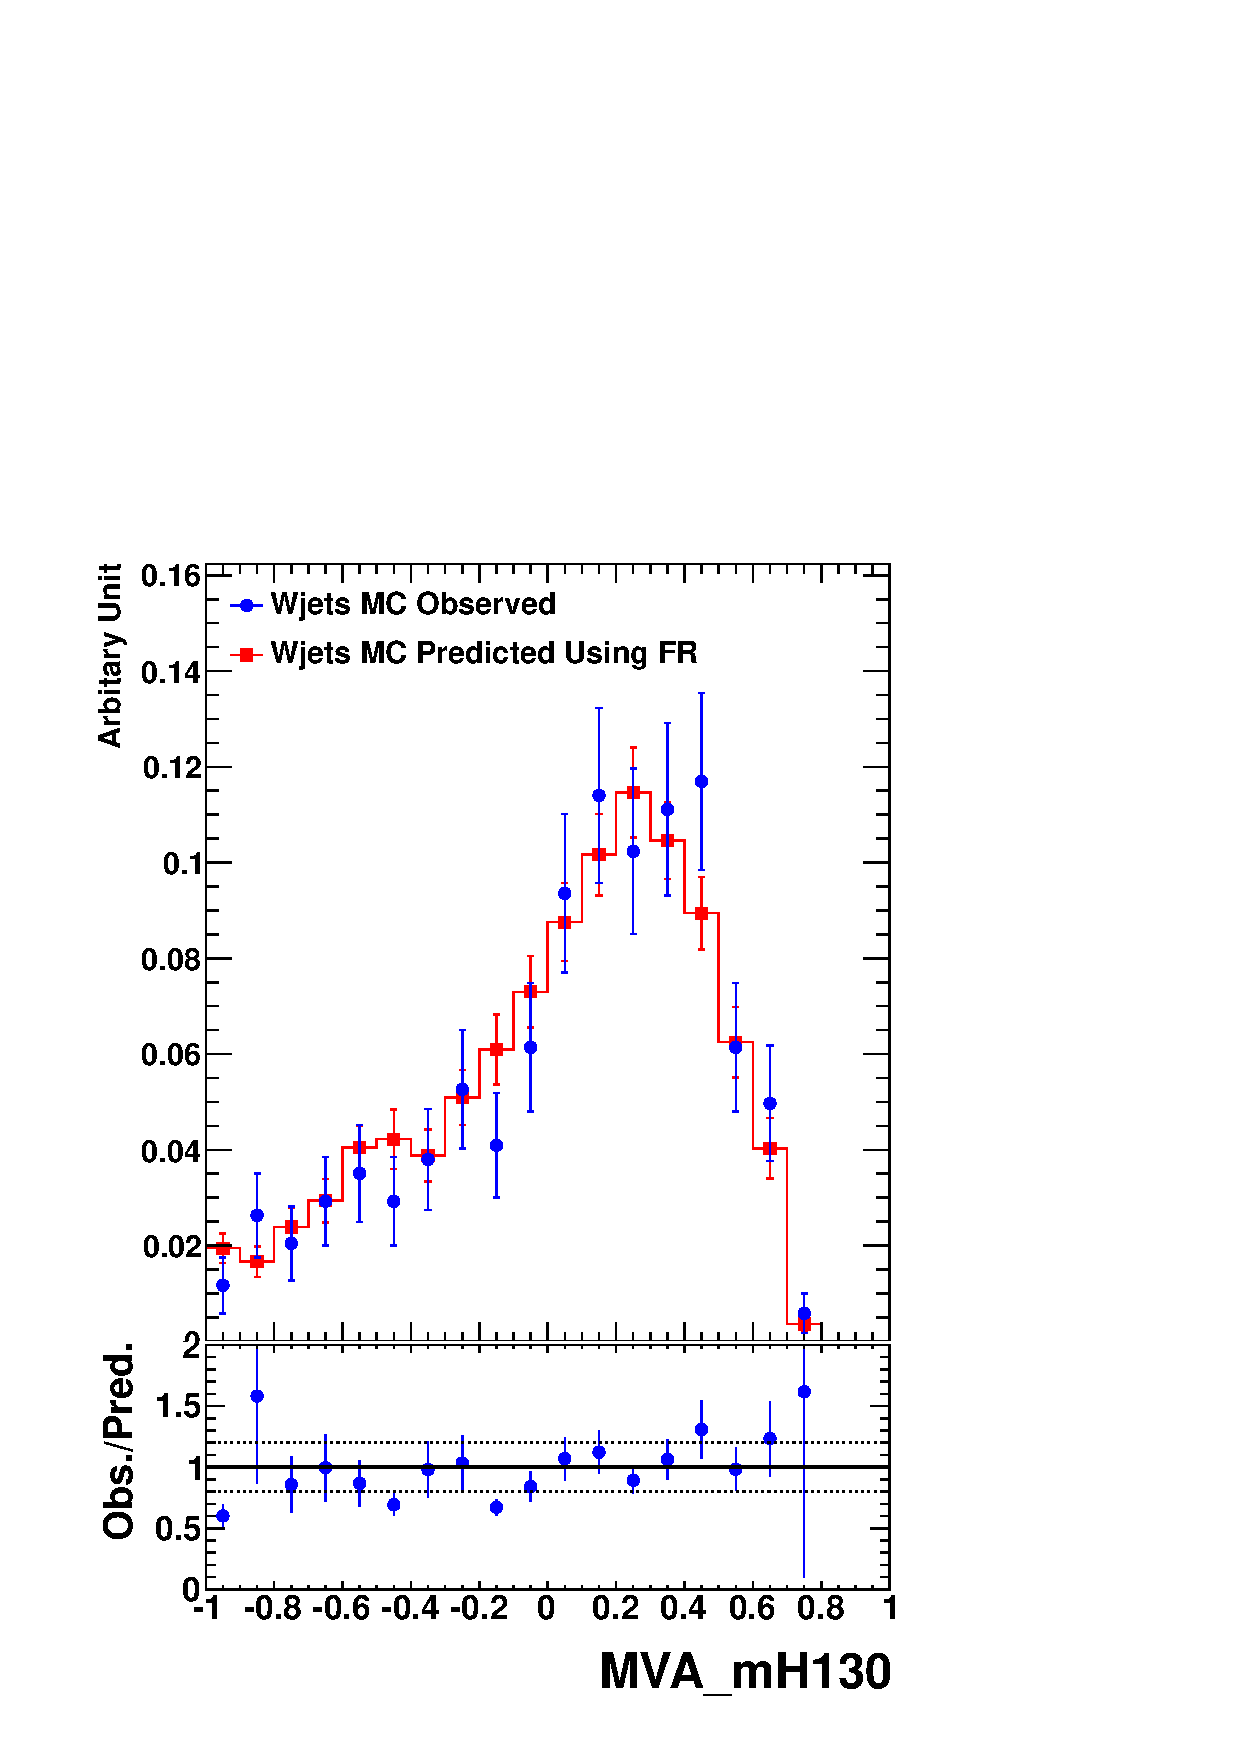
\includegraphics[width=0.3\textwidth]{figures/Wjets_MVA_MCClosure_mH130_0Jet.pdf}}
\subfigure[mH = 140]{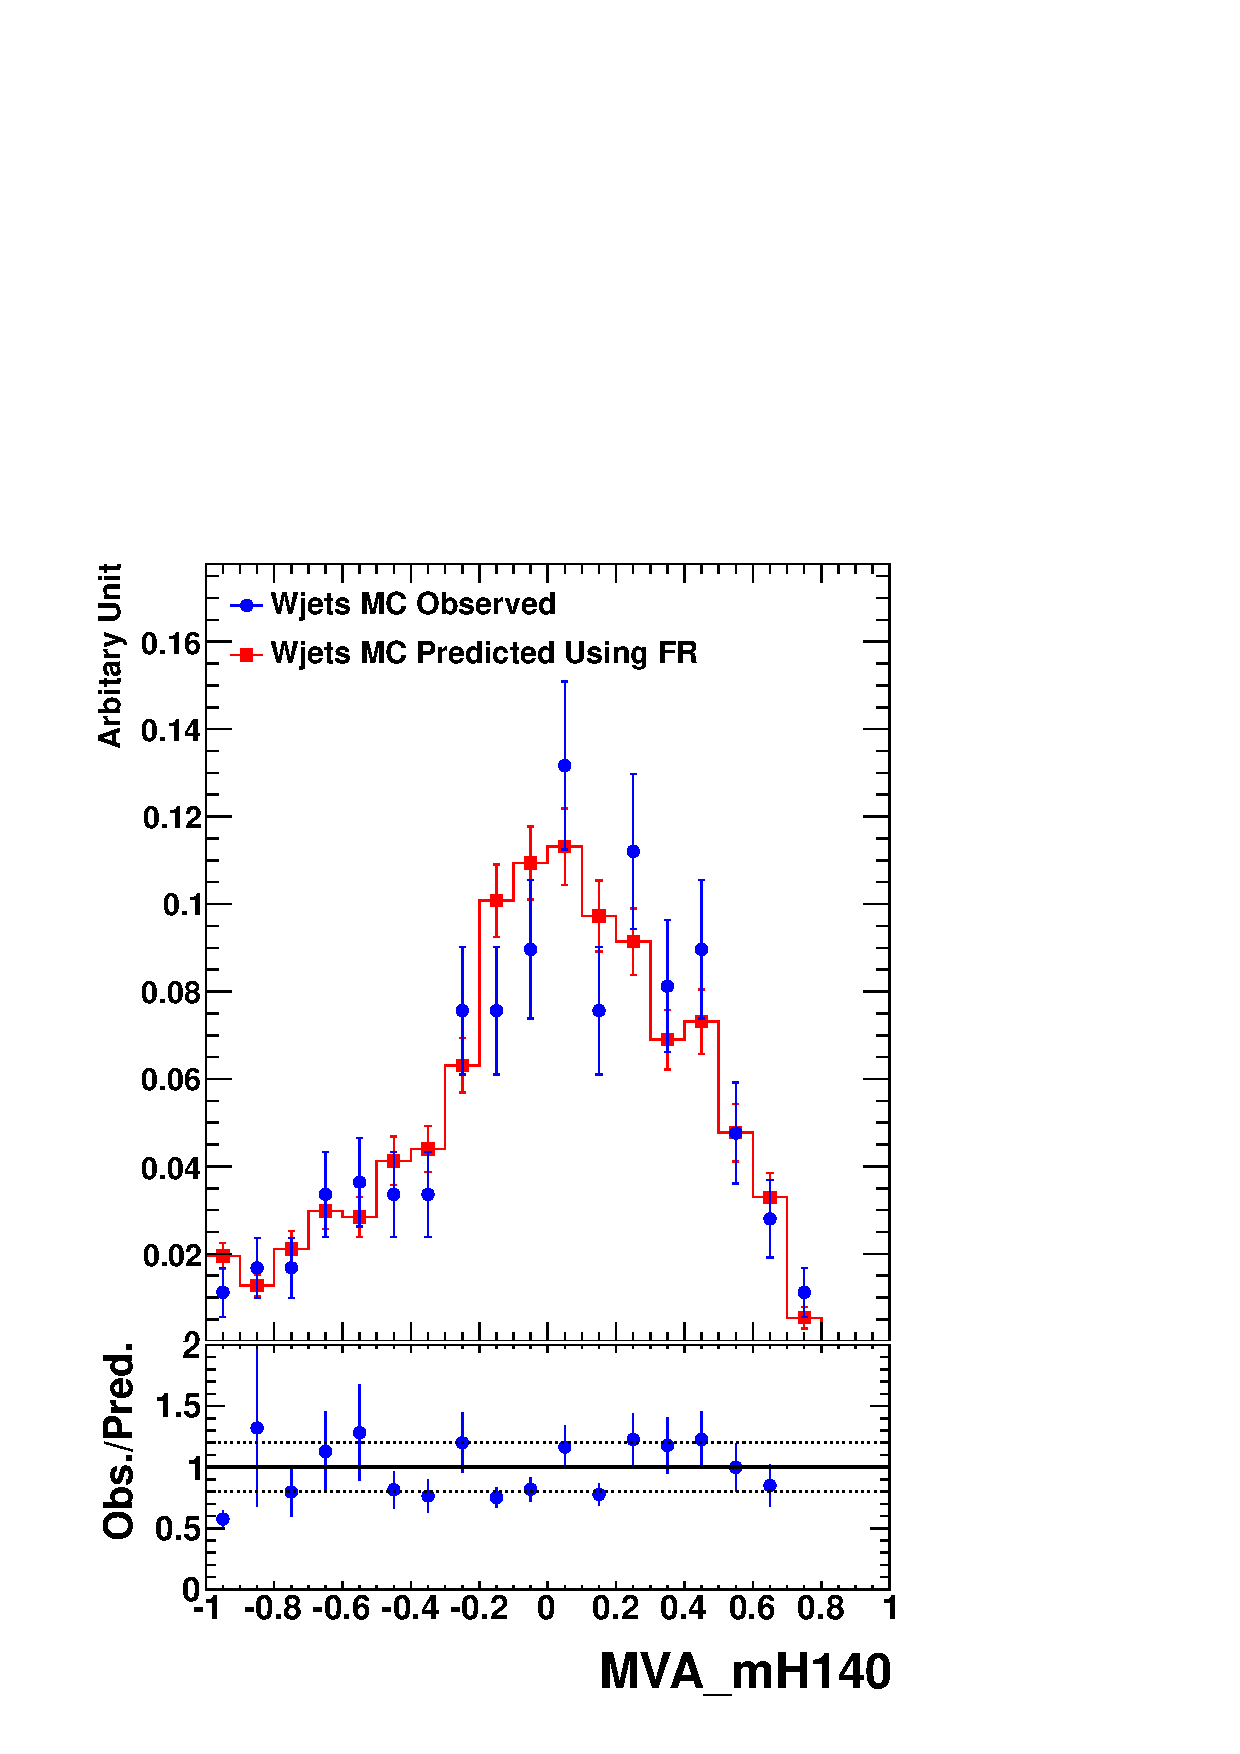
\includegraphics[width=0.3\textwidth]{figures/Wjets_MVA_MCClosure_mH140_0Jet.pdf}}\\
\subfigure[mH = 150]{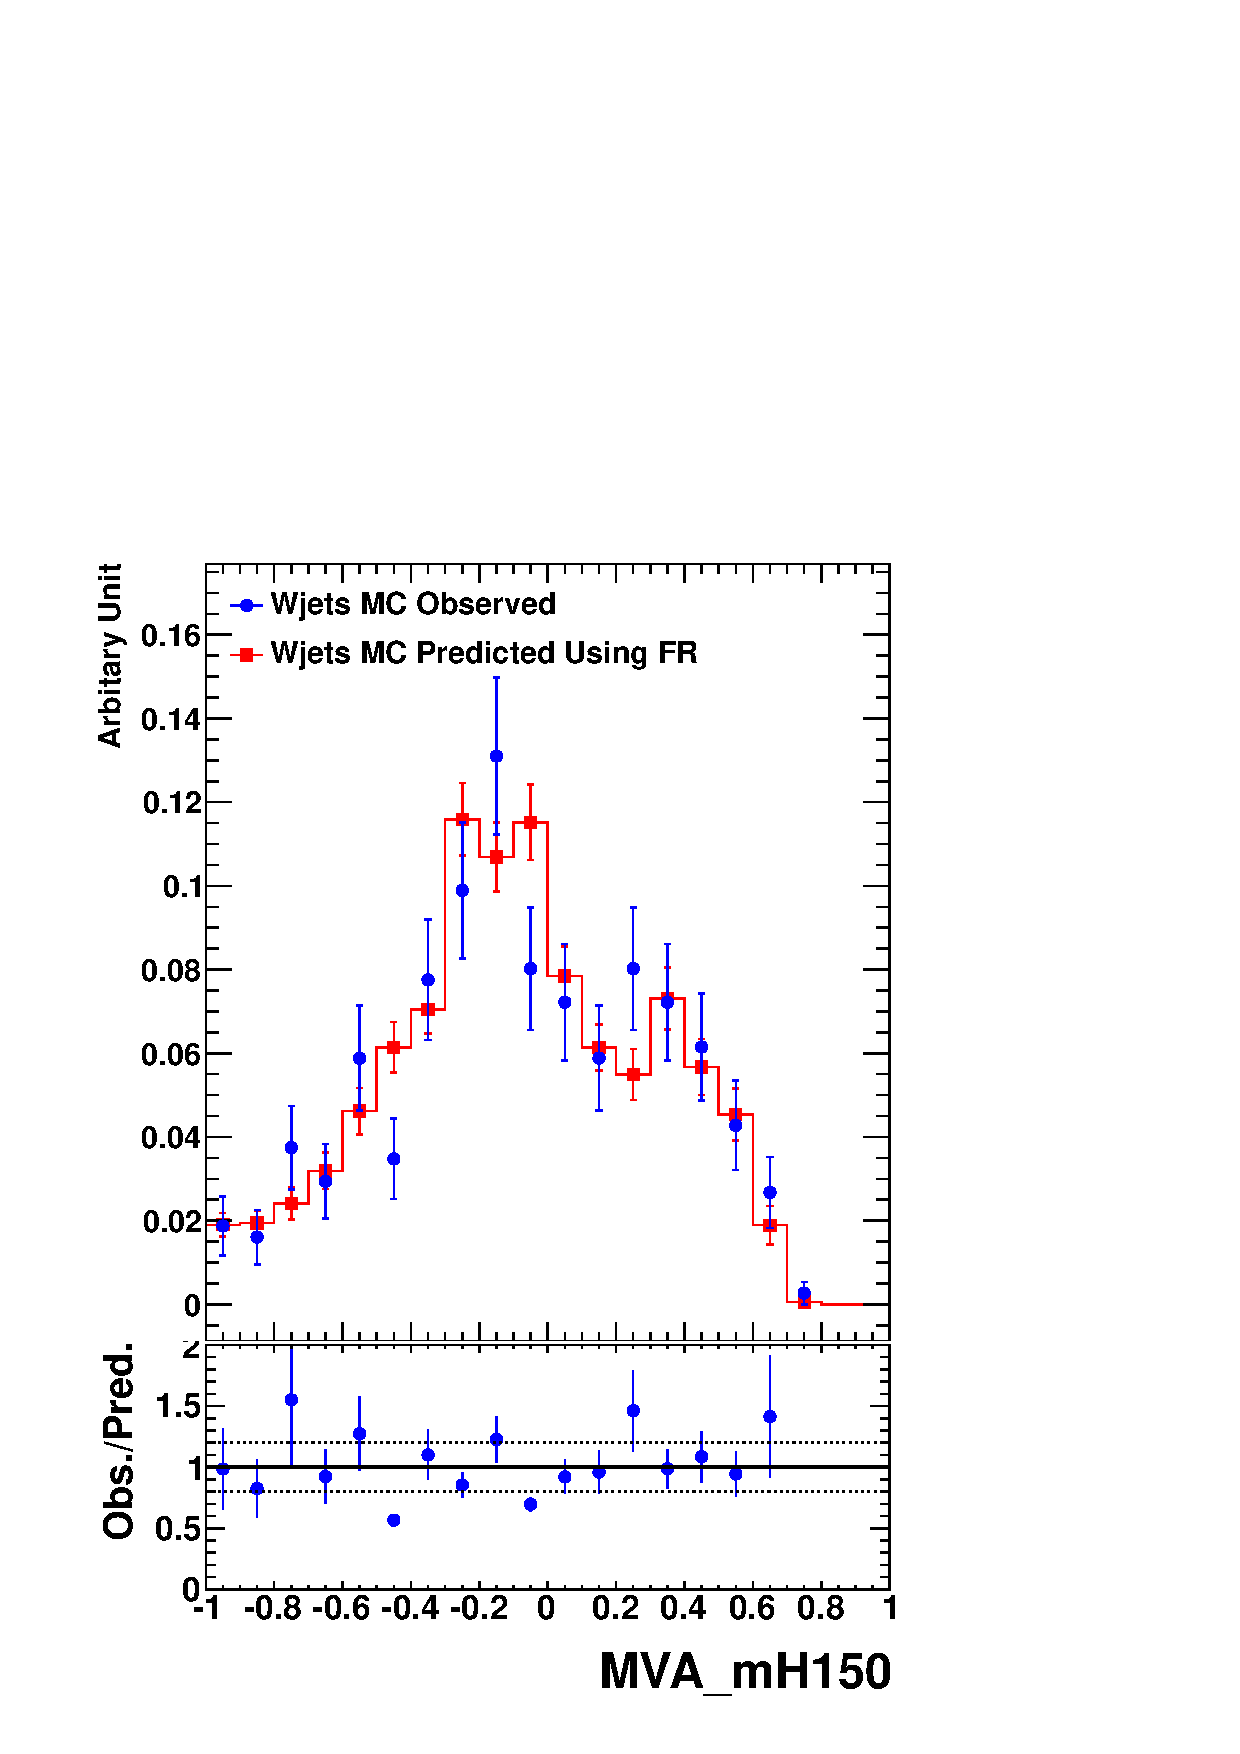
\includegraphics[width=0.3\textwidth]{figures/Wjets_MVA_MCClosure_mH150_0Jet.pdf}}
\subfigure[mH = 160]{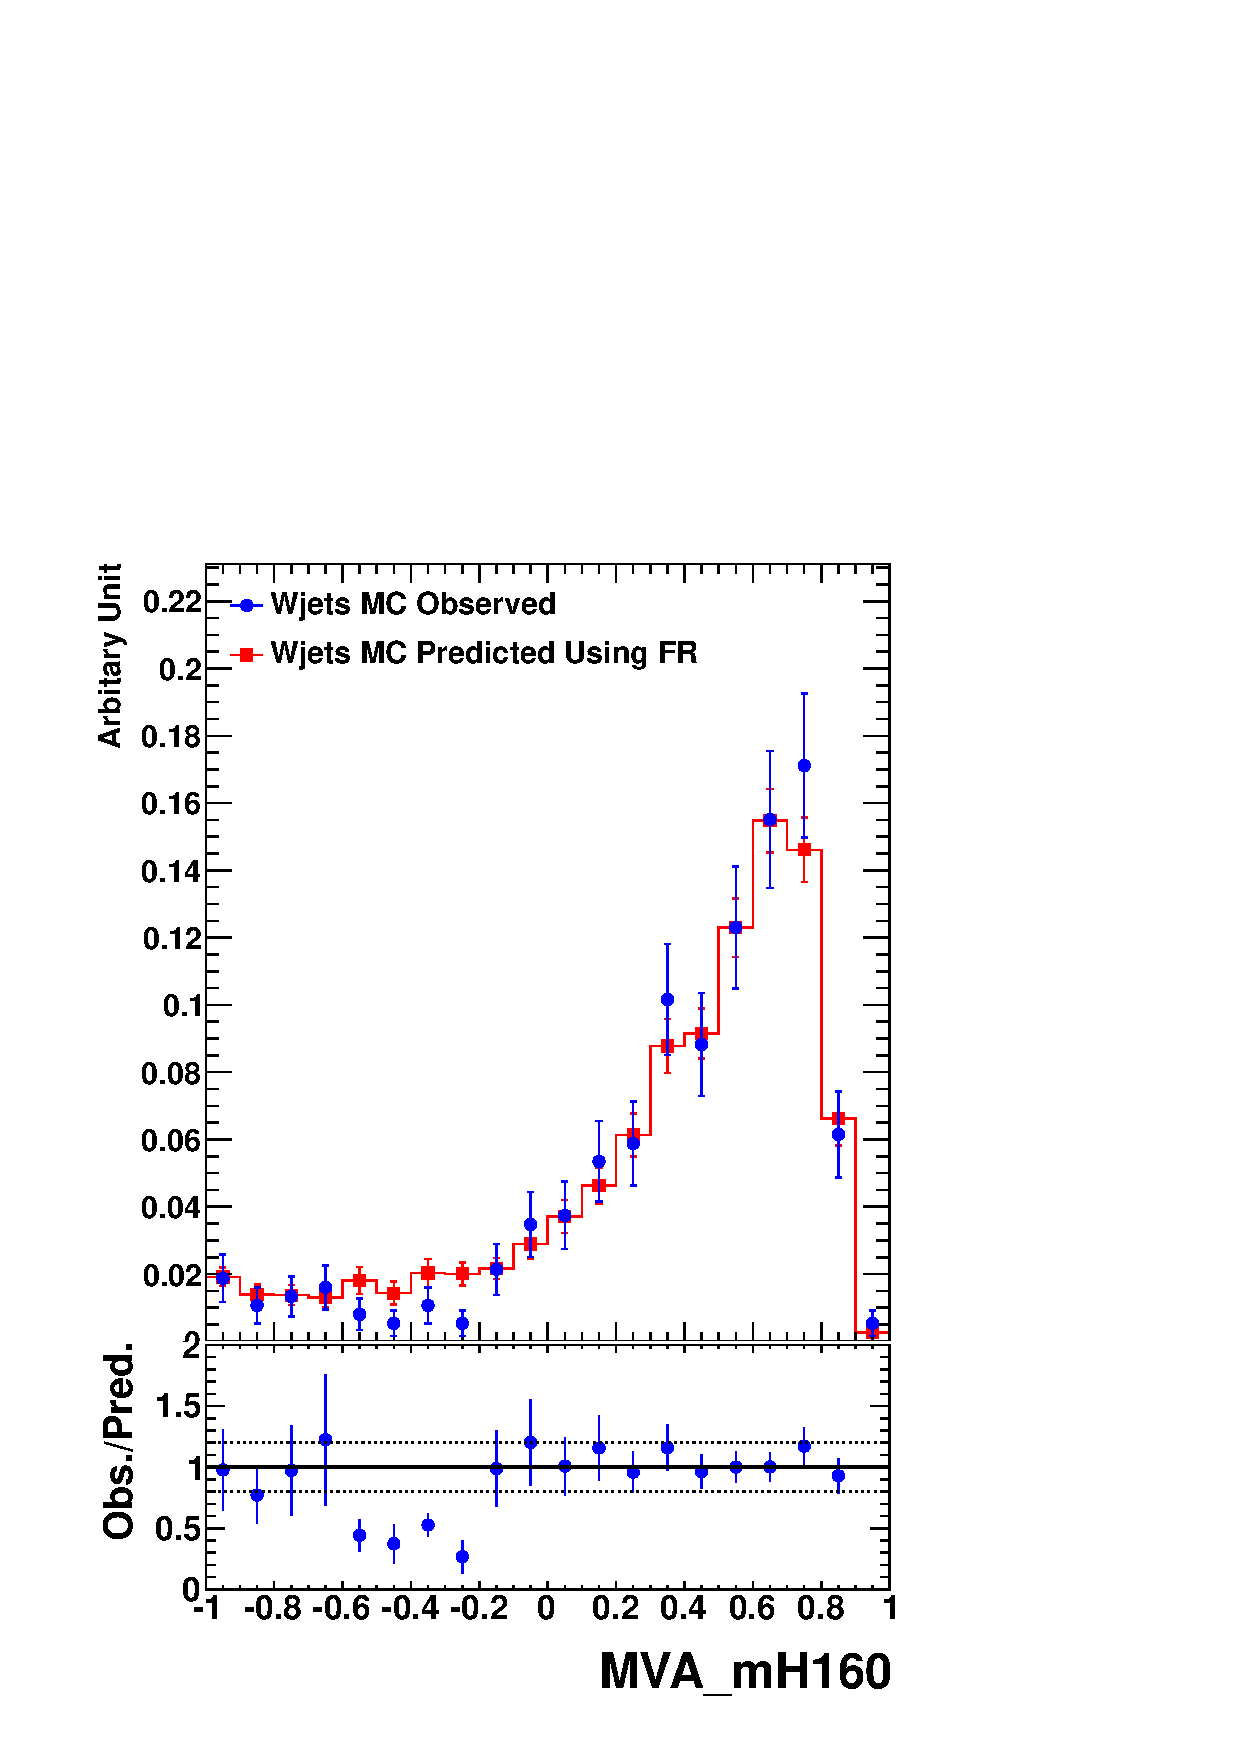
\includegraphics[width=0.3\textwidth]{figures/Wjets_MVA_MCClosure_mH160_0Jet.pdf}}
\subfigure[mH = 190]{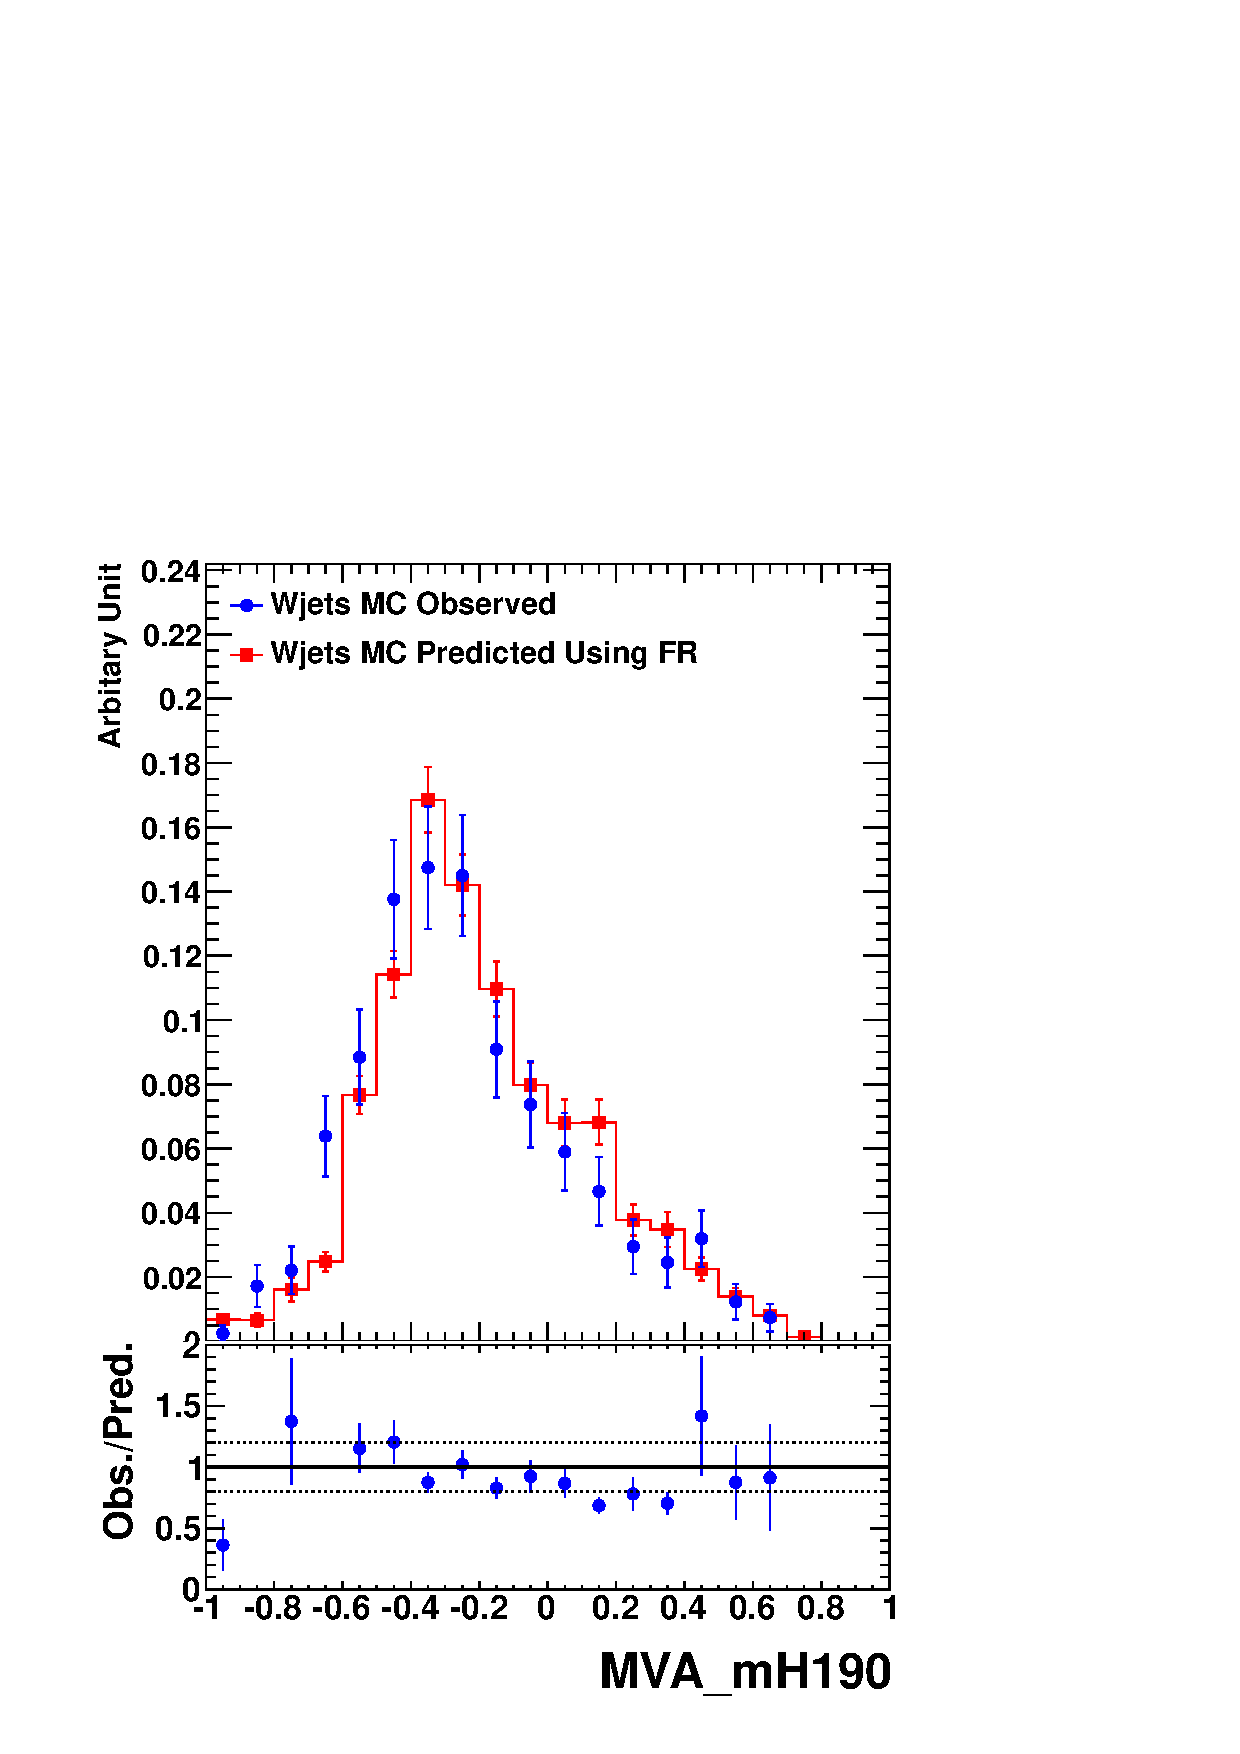
\includegraphics[width=0.3\textwidth]{figures/Wjets_MVA_MCClosure_mH190_0Jet.pdf}}\\
\subfigure[mH = 200]{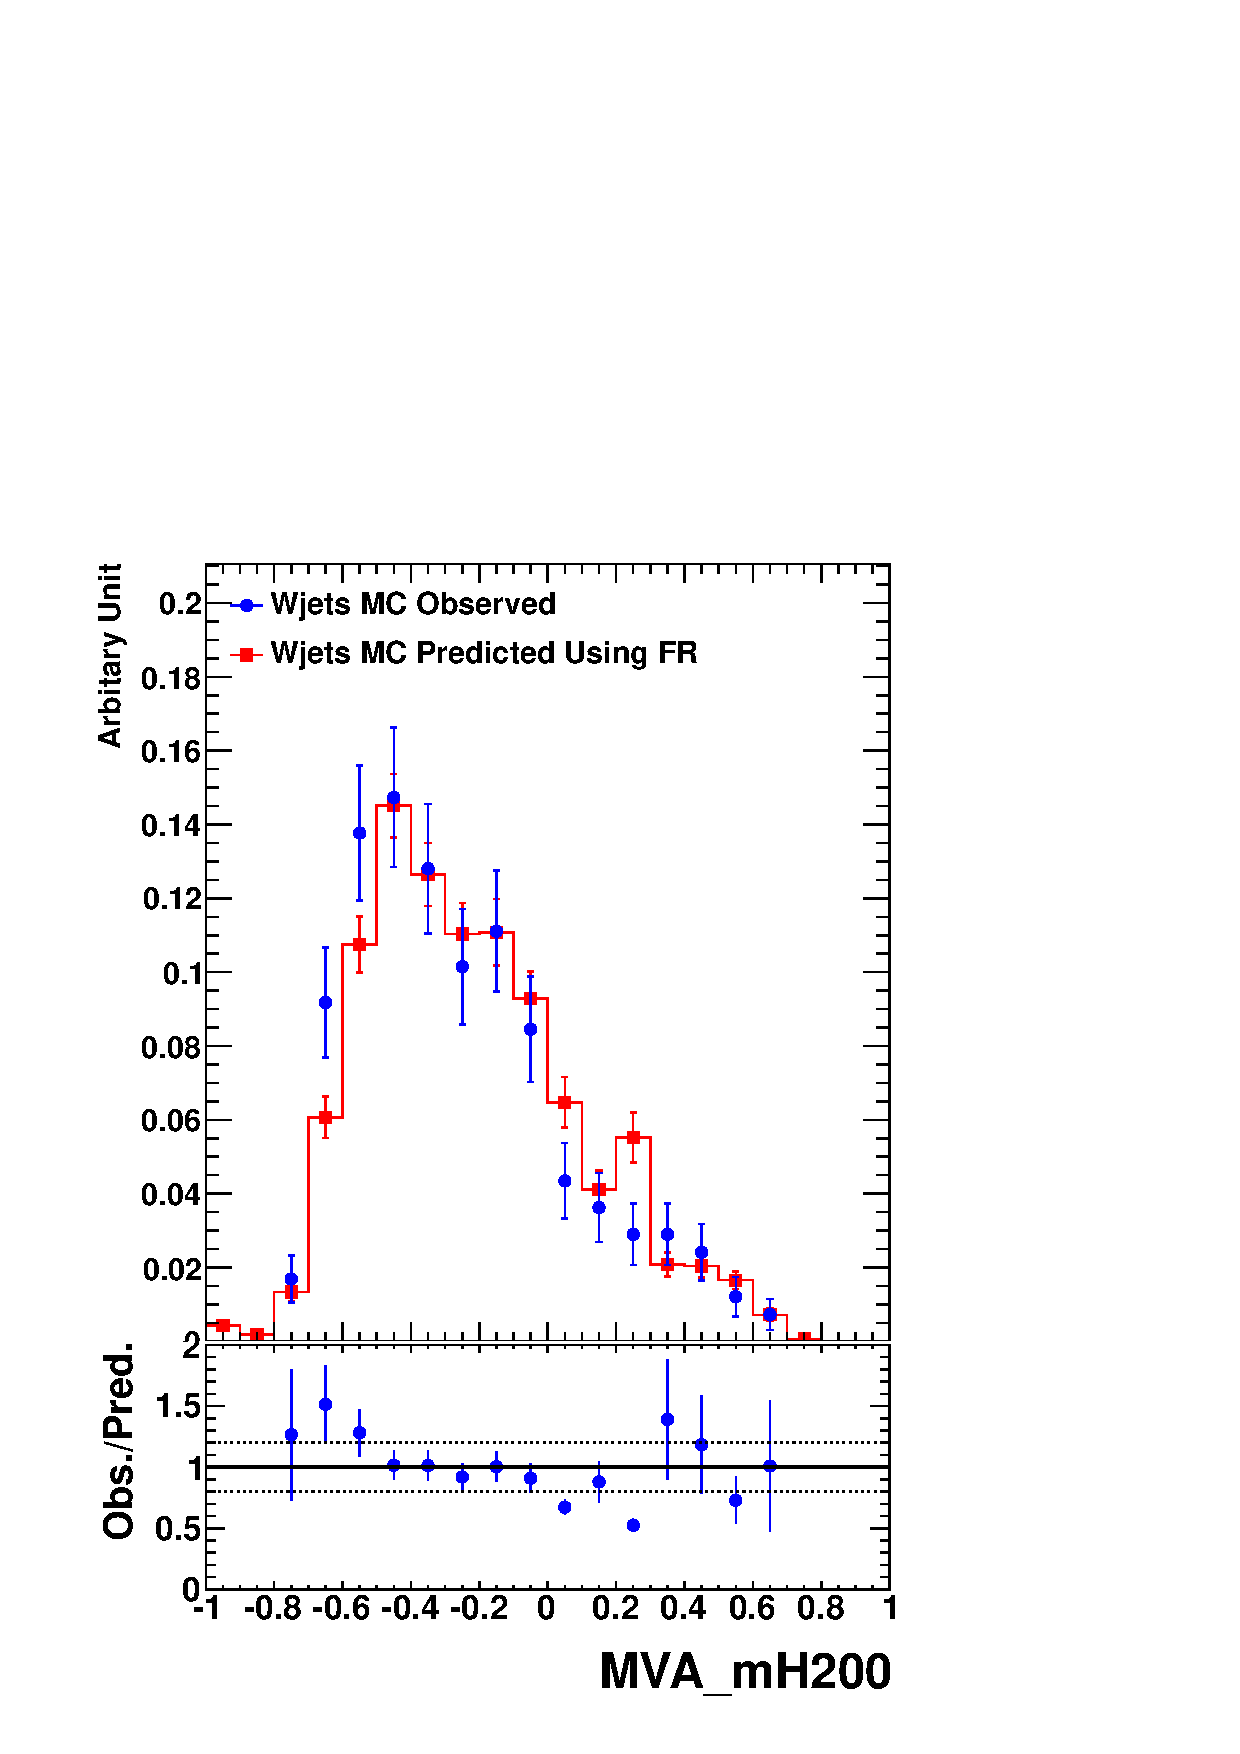
\includegraphics[width=0.3\textwidth]{figures/Wjets_MVA_MCClosure_mH200_0Jet.pdf}}
\subfigure[mH = 250]{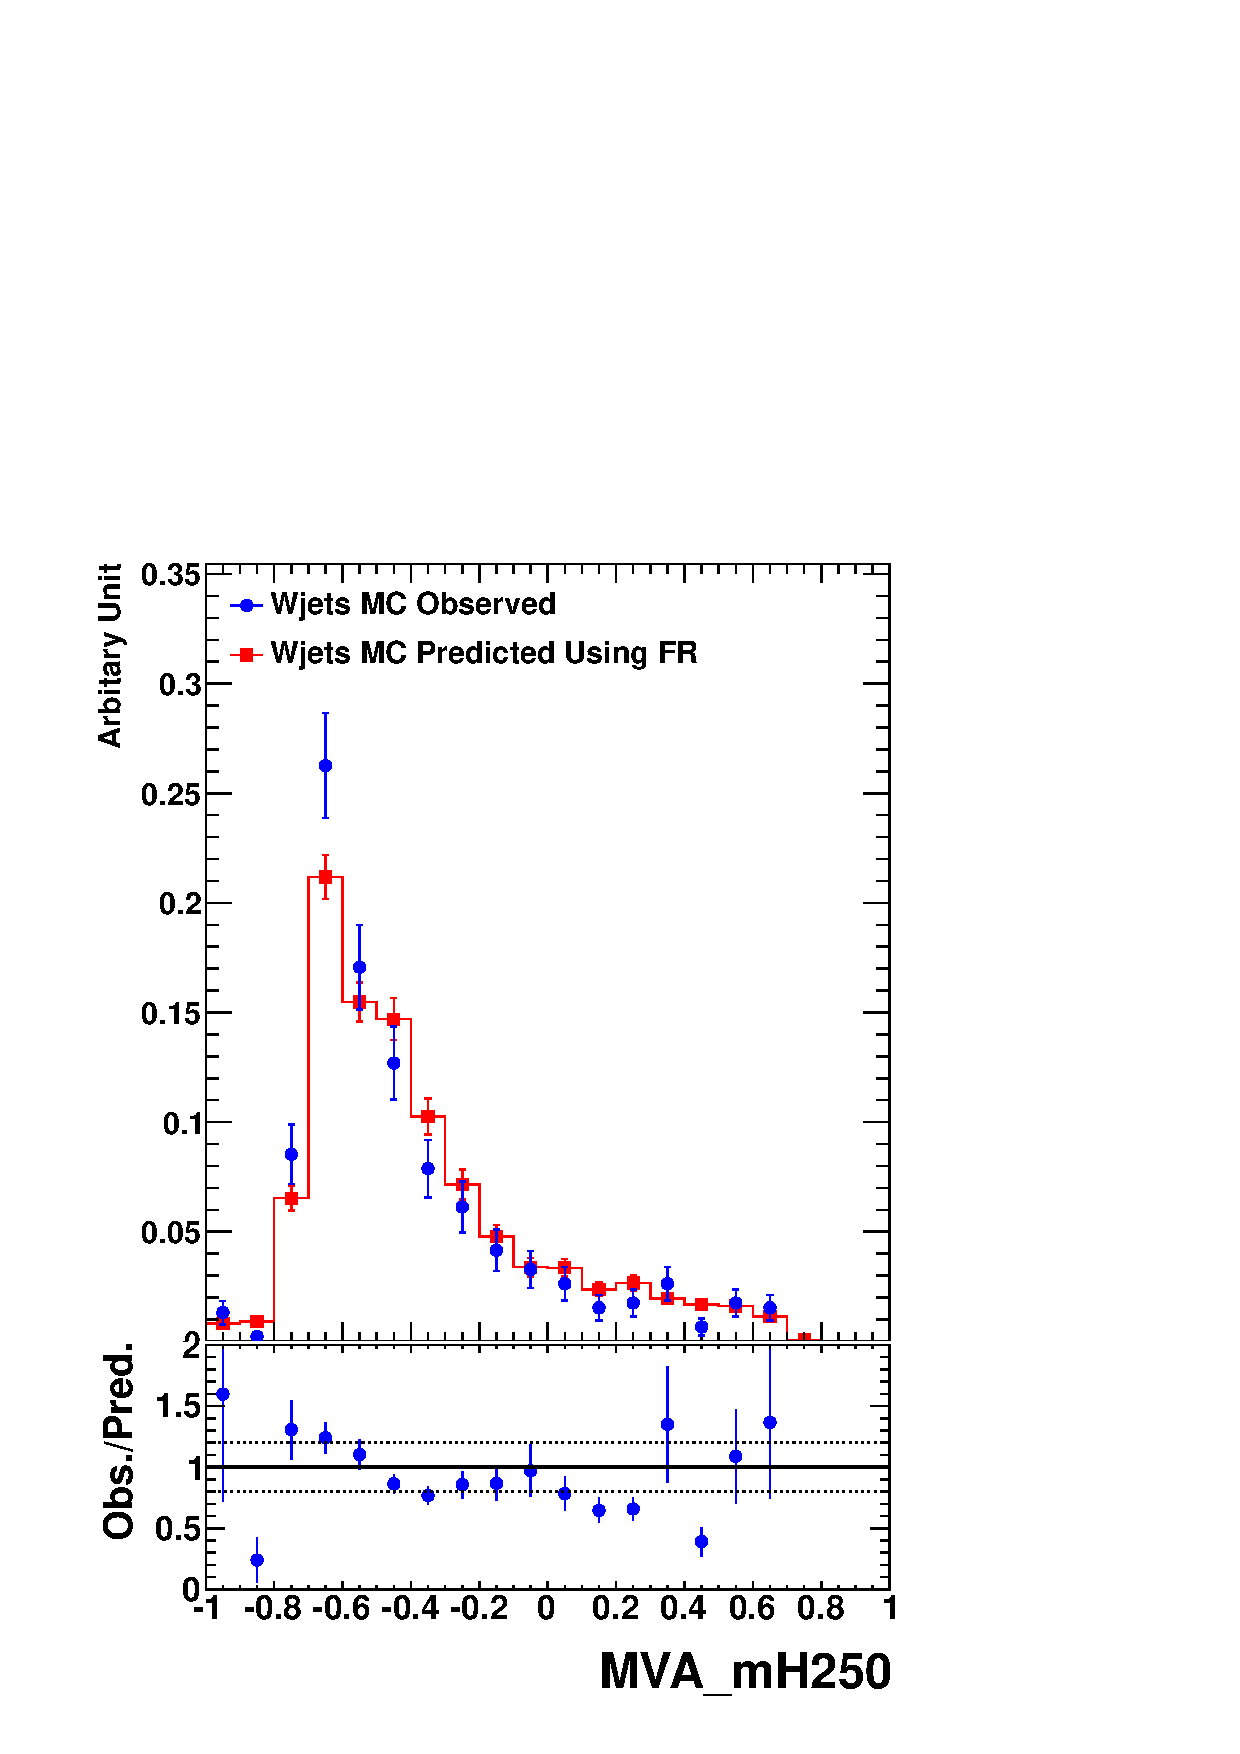
\includegraphics[width=0.3\textwidth]{figures/Wjets_MVA_MCClosure_mH250_0Jet.pdf}}
\subfigure[mH = 300]{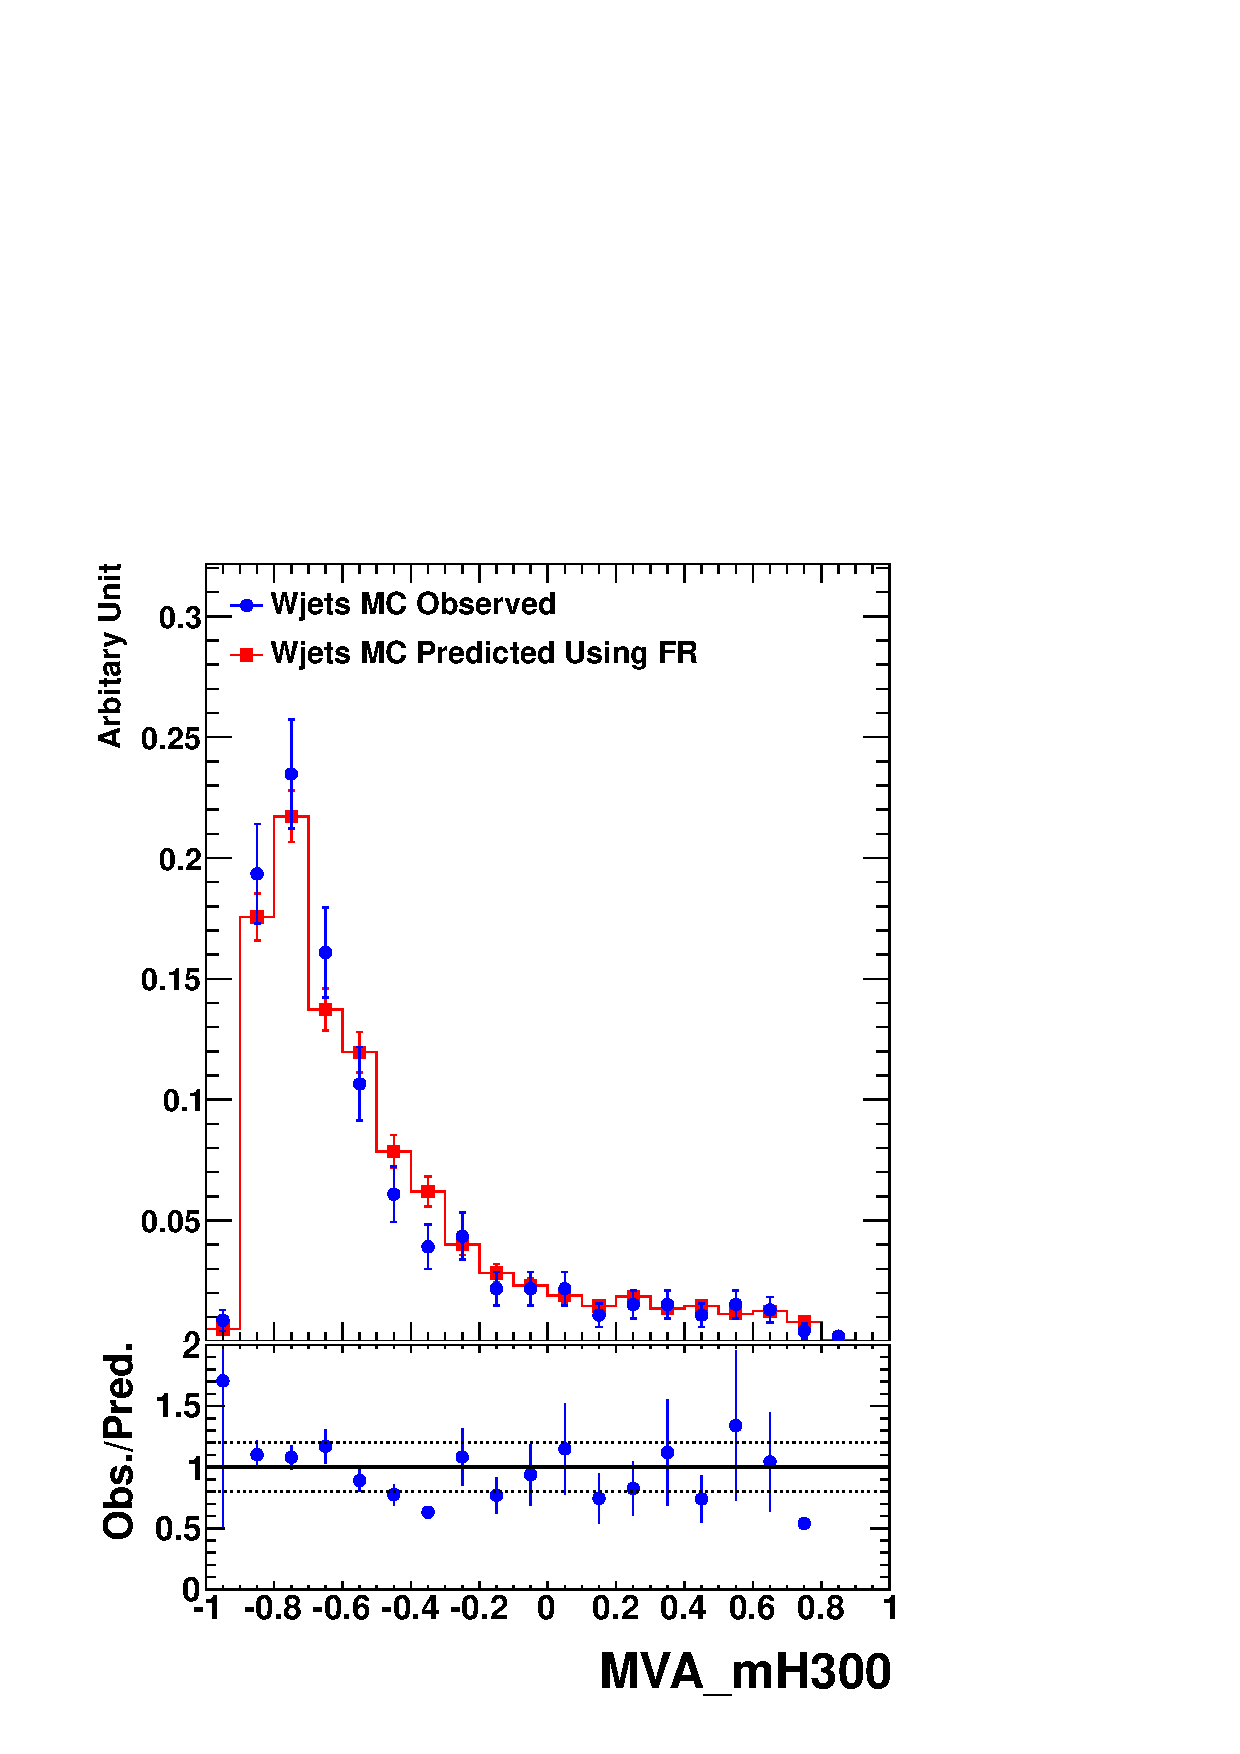
\includegraphics[width=0.3\textwidth]{figures/Wjets_MVA_MCClosure_mH300_0Jet.pdf}}\\
\caption{The $\Wjets$ MVA distributions at higgs signal regions estimated using $\Wjets$ MC. 
In each higgs region, we compare the MVA distribution predicted using data-driven method 
using events in the side-band region (solid square) with the MC estimation using events in the 
signal region (solid dot). The distributions are normalized to unity in both methods 
to assess the difference in the shape, shown as the ``Obs./Pred.''. 
}
\label{fig:wjetsshape_mcclosure}
\end{center}
\end{figure}
%%%%%%%%%%%%%%%%%%%%%%%%%%%%%%%%%%%5


